\documentclass{standalone}
\usepackage{tikz}
\usepackage{color}
\usetikzlibrary{positioning, shapes, arrows.meta, calc, decorations.pathreplacing}

\definecolor{myblue}{RGB}{82,126,171}
\definecolor{myred}{RGB}{168, 50, 50}

\tikzset{
  square/.style={draw,outer sep=5,inner sep=3,minimum size=10,line width=0, 
    very thick, draw=myblue, top color=white,bottom color=white},
  noborder/.style={draw,outer sep=0,inner sep=0,minimum size=20,line width=1, 
    draw=none, scale=1, anchor=west},
  blue/.style={draw,outer sep=35,inner sep=3,minimum size=20, line width=1, 
    very thick, draw=none, top color=myblue, bottom color=myblue, scale=1.25},
   noborderr/.style={draw,outer sep=0,inner sep=0,minimum size=20,line width=1, 
    draw=none, scale=1, anchor=west}
}

\begin{document}

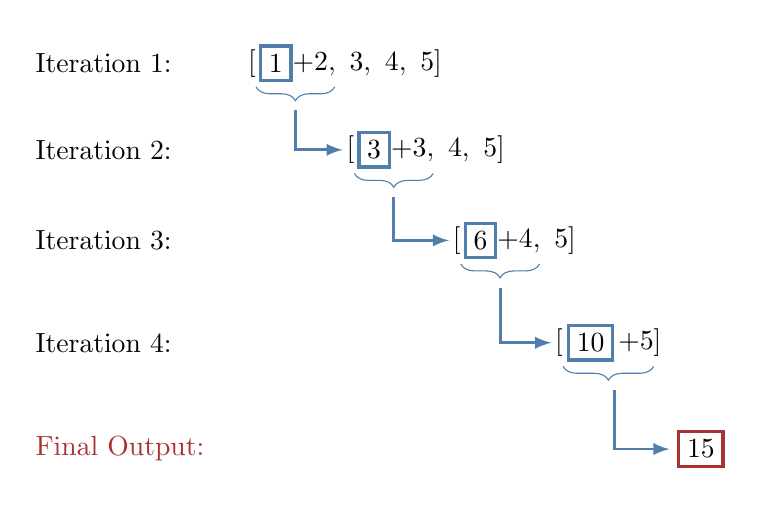
\begin{tikzpicture}[>={Latex[width=2mm,length=2mm]}]



\draw[decorate,color=myblue,decoration={brace,amplitude=5pt}] (-0.45,1.4) -- (-1.45,1.4);
\draw[-latex,line width=1 pt,color=myblue] (-0.95,1.1) |- (-0.35,0.6);

\node [noborderr] at (-1.55,1.7) {$[ ~~~~+ 2, ~3,~ 4, ~5]$};
\node [square] at (-1.2,1.7) {$1$};


\draw[decorate,color=myblue,decoration={brace,amplitude=5pt}] (0.8,0.3) -- (-0.2,0.3);
\draw[-latex,line width=1 pt, color=myblue] (0.3,0) |- (1,-0.55);

\node [noborderr] at (-0.3,0.6) {$[~~~~ + 3,~ 4, ~5]$};
\node [square] at (0.05,0.6) {$3$};


\draw[decorate,color=myblue,decoration={brace,amplitude=5pt}] (2.15,-0.85) -- (1.15,-0.85);
\draw[-latex,line width=1 pt,color=myblue] (1.65,-1.15) |- (2.3,-1.85);

\node [noborderr] at (1.05,-0.55) {$[~~~~ + 4, ~5]$};
\node [square] at (1.4,-0.55) {$6$};


\draw[decorate,color=myblue,decoration={brace,amplitude=5pt}] (3.6,-2.15) -- (2.45,-2.15);
\draw[-latex, line width=1 pt, color=myblue] (3.1,-2.45) |- (3.8,-3.2);

\node [noborderr] at (2.35,-1.85) {$[~~~~ ~~+ 5]$};
\node [square] at (2.8,-1.85) {$10$};
\node [square,draw=myred] at (4.2,-3.2) {$15$};

\node [noborderr] at (-4.25,1.7) {Iteration 1:};
\node [noborderr] at (-4.25,0.6) {Iteration 2:};
\node [noborderr] at (-4.25,-0.55) {Iteration 3:};
\node [noborderr] at (-4.25,-1.85) {Iteration 4:};
\node [noborderr, color=myred] at (-4.25,-3.2) {Final Output:};



\usetikzlibrary{calc}
\pgftransformreset
\node[inner sep=0pt,outer sep=0pt,minimum size=0pt,line width=0pt,text width=0pt,text height=0pt] at (current bounding box) {};
%add border to avoid cropping by pdflibnet
\foreach \border in {0.1}
  \useasboundingbox (current bounding box.south west)+(-\border,-\border) rectangle (current bounding box.north east)+(\border,\border);
\newwrite\metadatafile
\immediate\openout\metadatafile=\jobname_BB.txt
\path
  let
    \p1=(current bounding box.south west),
    \p2=(current bounding box.north east)
  in
  node[inner sep=0pt,outer sep=0pt,minimum size=0pt,line width=0pt,text width=0pt,text height=0pt,draw=white] at (current bounding box) {
\immediate\write\metadatafile{\p1,\p2}
};
\immediate\closeout\metadatafile
\end{tikzpicture}

\end{document}

